%%%%%%%%%%%%%%%%%%%%%%%%%%%%%%%%%%%%%%%%%%%%%%%%%%%%%%%%%%%%%%%%%%%%%
%                                                                   %
%	CHAPTER THREE, SOFTWARE AND API                                   %
%                                                                   %
%%%%%%%%%%%%%%%%%%%%%%%%%%%%%%%%%%%%%%%%%%%%%%%%%%%%%%%%%%%%%%%%%%%%%

\chapter{Software in HPC}

\section{Introduction}
After presenting the rules of HPC and the hardware that compose the cluster, we introduce the most famous ways to target those architectures and supercomputers with programming models.
Then, fitting those models, we present the possible options in the language, the API, the distribution and the accelerators code. 

This chapter details the most important programming models and the software options for HPC programming and include the choices we made for our applications.
Then it presents the software used to benchmark the supercomputers. 
We present here the most famous, the TOP500, GRAPH500, HPGC and GREEN500 to give their advantages and weaknesses. 

\section{Parallel and distributed programming Models}
\index{Random Access Machine}
The Flynn taxonomy developed in chapter 1 was a characterization of the executions models. 
This model can be extended to programming models which are an extension of MIMD. 
We consider here a \textit{Random Access Machine} (RAM). 
The memory of this machine consists of an unbounded sequence of registers each of which may hold an integer value. 
In this model the applications can access to every memory words directly in write or read manner.
There is three main operations: load from memory to register; compute operation between data; store from register to memory. 
This model is use to estimate the complexity of sequential algorithms. 
If we consider the unit of time of each operation (like in cycle) we can have an idea of the overall time of the application.
We identify two types of RAM, the Parallel-RAM using shared memory and the Distributed-RAM using distributed memory. 

\subsection{Parallel Random Access Machine}
\index{Parallel Random Access Machine}
The Parallel Random Access Machine \cite{fortune1978parallelism}, PRAM, is a model in which the global memory is shared between the processes and each process have its own local memory/registers.
The execution is synchronous, processes execute the same instructions at the same time. 
In this model each process is identify with its own index enabling to target different data. 
The problem in this model will be the concurrency in reading (R) and writing (W) data as the memory is shared between the processes.
Indeed, mutual exclusion have to be set with exclusive (E) or concurrent (C) behaviors and we find 4 combinations: EREW, ERCW, CREW and CRCW.
As the reading is not critical for data concurrency the standard model will be Concurrent Reading and Exclusive Writing: CREW.

\begin{figure}[t!]
\centering
\resizebox {\columnwidth} {!} {
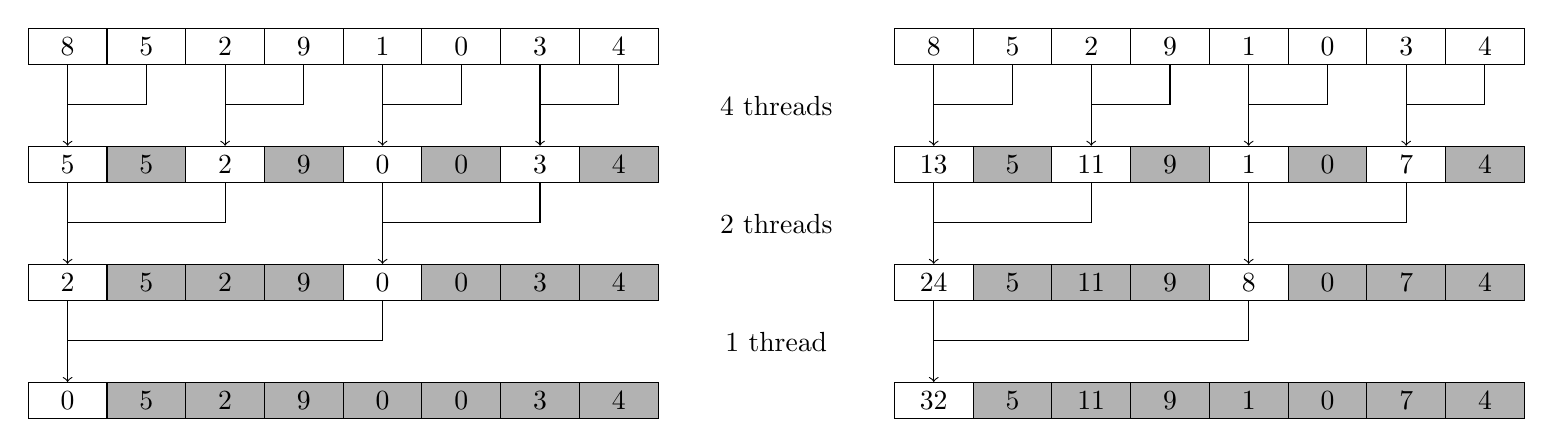
\begin{tikzpicture}
\def\i{4.5}
\node[draw,minimum width=1cm] (n00) at (0,\i) {8};
\node[draw,minimum width=1cm] (n01) at (1,\i) {5};
\node[draw,minimum width=1cm] (n02) at (2,\i) {2};
\node[draw,minimum width=1cm] (n03) at (3,\i) {9};
\node[draw,minimum width=1cm] (n04) at (4,\i) {1};
\node[draw,minimum width=1cm] (n05) at (5,\i) {0};
\node[draw,minimum width=1cm] (n06) at (6,\i) {3};
\node[draw,minimum width=1cm] (n07) at (7,\i) {4};
\def\i{3}
\node[draw,minimum width=1cm] (n10) at (0,\i) {5};
\node[draw,minimum width=1cm,fill=black!30] (n11) at (1,\i) {5};
\node[draw,minimum width=1cm] (n12) at (2,\i) {2};
\node[draw,minimum width=1cm,fill=black!30] (n13) at (3,\i) {9};
\node[draw,minimum width=1cm] (n14) at (4,\i) {0};
\node[draw,minimum width=1cm,fill=black!30] (n15) at (5,\i) {0};
\node[draw,minimum width=1cm] (n16) at (6,\i) {3};
\node[draw,minimum width=1cm,fill=black!30] (n17) at (7,\i) {4};
\def\i{1.5}
\node[draw,minimum width=1cm] (n20) at (0,\i) {2};
\node[draw,minimum width=1cm,fill=black!30] (n21) at (1,\i) {5};
\node[draw,minimum width=1cm,fill=black!30] (n22) at (2,\i) {2};
\node[draw,minimum width=1cm,fill=black!30] (n23) at (3,\i) {9};
\node[draw,minimum width=1cm] (n24) at (4,\i) {0};
\node[draw,minimum width=1cm,fill=black!30] (n25) at (5,\i) {0};
\node[draw,minimum width=1cm,fill=black!30] (n26) at (6,\i) {3};
\node[draw,minimum width=1cm,fill=black!30] (n27) at (7,\i) {4};
\def\i{0}
\node[draw,minimum width=1cm] (n30) at (0,\i) {0};
\node[draw,minimum width=1cm,fill=black!30] (n31) at (1,\i) {5};
\node[draw,minimum width=1cm,fill=black!30] (n32) at (2,\i) {2};
\node[draw,minimum width=1cm,fill=black!30] (n33) at (3,\i) {9};
\node[draw,minimum width=1cm,fill=black!30] (n34) at (4,\i) {0};
\node[draw,minimum width=1cm,fill=black!30] (n35) at (5,\i) {0};
\node[draw,minimum width=1cm,fill=black!30] (n36) at (6,\i) {3};
\node[draw,minimum width=1cm,fill=black!30] (n37) at (7,\i) {4};
% Add the arrows 
\draw[->] (n00.south) -- (n10.north);
\draw[-] (n01.south) -- ([yshift=-.5cm]n01.south) -- ([yshift=-.5cm]n00.south);
\draw[->] (n02.south) -- (n12.north);
\draw[-] (n03.south) -- ([yshift=-.5cm]n03.south) -- ([yshift=-.5cm]n02.south);
\draw[->] (n04.south) -- (n14.north);
\draw[-] (n05.south) -- ([yshift=-.5cm]n05.south) -- ([yshift=-.5cm]n04.south);
\draw[->] (n06.south) -- (n16.north);
\draw[-] (n07.south) -- ([yshift=-.5cm]n07.south) -- ([yshift=-.5cm]n06.south);

\draw[->] (n10.south) -- (n20.north);
\draw[-] (n12.south) -- ([yshift=-.5cm]n12.south) -- ([yshift=-.5cm]n10.south);
\draw[->] (n14.south) -- (n24.north);
\draw[-] (n16.south) -- ([yshift=-.5cm]n16.south) -- ([yshift=-.5cm]n14.south);

\draw[->] (n20.south) -- (n30.north);
\draw[-] (n24.south) -- ([yshift=-.5cm]n24.south) -- ([yshift=-.5cm]n20.south);


\def\i{4.5}
\node[draw,minimum width=1cm] (n00) at (11,\i) {8};
\node[draw,minimum width=1cm] (n01) at (12,\i) {5};
\node[draw,minimum width=1cm] (n02) at (13,\i) {2};
\node[draw,minimum width=1cm] (n03) at (14,\i) {9};
\node[draw,minimum width=1cm] (n04) at (15,\i) {1};
\node[draw,minimum width=1cm] (n05) at (16,\i) {0};
\node[draw,minimum width=1cm] (n06) at (17,\i) {3};
\node[draw,minimum width=1cm] (n07) at (18,\i) {4};
\def\i{3}
\node[draw,minimum width=1cm] (n10) at (11,\i) {13};
\node[draw,minimum width=1cm,fill=black!30] (n11) at (12,\i) {5};
\node[draw,minimum width=1cm] (n12) at (13,\i) {11};
\node[draw,minimum width=1cm,fill=black!30] (n13) at (14,\i) {9};
\node[draw,minimum width=1cm] (n14) at (15,\i) {1};
\node[draw,minimum width=1cm,fill=black!30] (n15) at (16,\i) {0};
\node[draw,minimum width=1cm] (n16) at (17,\i) {7};
\node[draw,minimum width=1cm,fill=black!30] (n17) at (18,\i) {4};
\def\i{1.5}
\node[draw,minimum width=1cm] (n20) at (11,\i) {24};
\node[draw,minimum width=1cm,fill=black!30] (n21) at (12,\i) {5};
\node[draw,minimum width=1cm,fill=black!30] (n22) at (13,\i) {11};
\node[draw,minimum width=1cm,fill=black!30] (n23) at (14,\i) {9};
\node[draw,minimum width=1cm] (n24) at (15,\i) {8};
\node[draw,minimum width=1cm,fill=black!30] (n25) at (16,\i) {0};
\node[draw,minimum width=1cm,fill=black!30] (n26) at (17,\i) {7};
\node[draw,minimum width=1cm,fill=black!30] (n27) at (18,\i) {4};
\def\i{0}
\node[draw,minimum width=1cm] (n30) at (11,\i) {32};
\node[draw,minimum width=1cm,fill=black!30] (n31) at (12,\i) {5};
\node[draw,minimum width=1cm,fill=black!30] (n32) at (13,\i) {11};
\node[draw,minimum width=1cm,fill=black!30] (n33) at (14,\i) {9};
\node[draw,minimum width=1cm,fill=black!30] (n34) at (15,\i) {1};
\node[draw,minimum width=1cm,fill=black!30] (n35) at (16,\i) {0};
\node[draw,minimum width=1cm,fill=black!30] (n36) at (17,\i) {7};
\node[draw,minimum width=1cm,fill=black!30] (n37) at (18,\i) {4};
% Add the arrows 
\draw[->] (n00.south) -- (n10.north);
\draw[-] (n01.south) -- ([yshift=-.5cm]n01.south) -- ([yshift=-.5cm]n00.south);
\draw[->] (n02.south) -- (n12.north);
\draw[-] (n03.south) -- ([yshift=-.5cm]n03.south) -- ([yshift=-.5cm]n02.south);
\draw[->] (n04.south) -- (n14.north);
\draw[-] (n05.south) -- ([yshift=-.5cm]n05.south) -- ([yshift=-.5cm]n04.south);
\draw[->] (n06.south) -- (n16.north);
\draw[-] (n07.south) -- ([yshift=-.5cm]n07.south) -- ([yshift=-.5cm]n06.south);

\draw[->] (n10.south) -- (n20.north);
\draw[-] (n12.south) -- ([yshift=-.5cm]n12.south) -- ([yshift=-.5cm]n10.south);
\draw[->] (n14.south) -- (n24.north);
\draw[-] (n16.south) -- ([yshift=-.5cm]n16.south) -- ([yshift=-.5cm]n14.south);

\draw[->] (n20.south) -- (n30.north);
\draw[-] (n24.south) -- ([yshift=-.5cm]n24.south) -- ([yshift=-.5cm]n20.south);

% Text 
\node at (9,3.75) {4 threads};
\node at (9,2.25) {2 threads};
\node at (9,.75) {1 thread};

\end{tikzpicture}
}
\caption[PRAM model example]{PRAM model example on minimum and reduction computation. These reductions for $n$ values are performed in $log(n)$ steps and $n-1$ operations. }
\label{fig:pram_reduction}
\end{figure}

An example of PRAM model applied on a reduction is given on figure~\ref{fig:pram_reduction}.
In this example the computation of minimum, maximum or a reduction can be perform on an array of $n$ values in $log(n)$ steps and $n-1$ operations.
This kind of reduction or scan are used to reach performances on multi-core and many-core code in this study.
We will give example of those reductions in different languages and API. 

\subsection{Distributed Random Access Machine}
\index{Distributed Random Access Machine}
\index{No Remote Memory Access}
For machine that base their memory model on NoRMA the execution model can be qualify of Distributed Random Access Machine, DRAM.
It is based on NoRMA memories detailed in part \ref{sec:NORMA}.
This model is in opposition to PRAM because the synchronization between processes is made by communications and messages. 
Those communications can be of several kind and depend of physical architecture, interconnection network and software used.

\subsection{H-PRAM}
\index{Hybrid Parallel Randon Access Machine}
A DRAM can be composed of an ensemble of PRAM system interconnected. 
Each of them working on their own data and instructions. 
This is an intermediate model between PRAM and DRAM having a set of shared memory and synchronous execution, the overall execution being asynchronous and having distributed memory.

\begin{figure}
\begin{center}
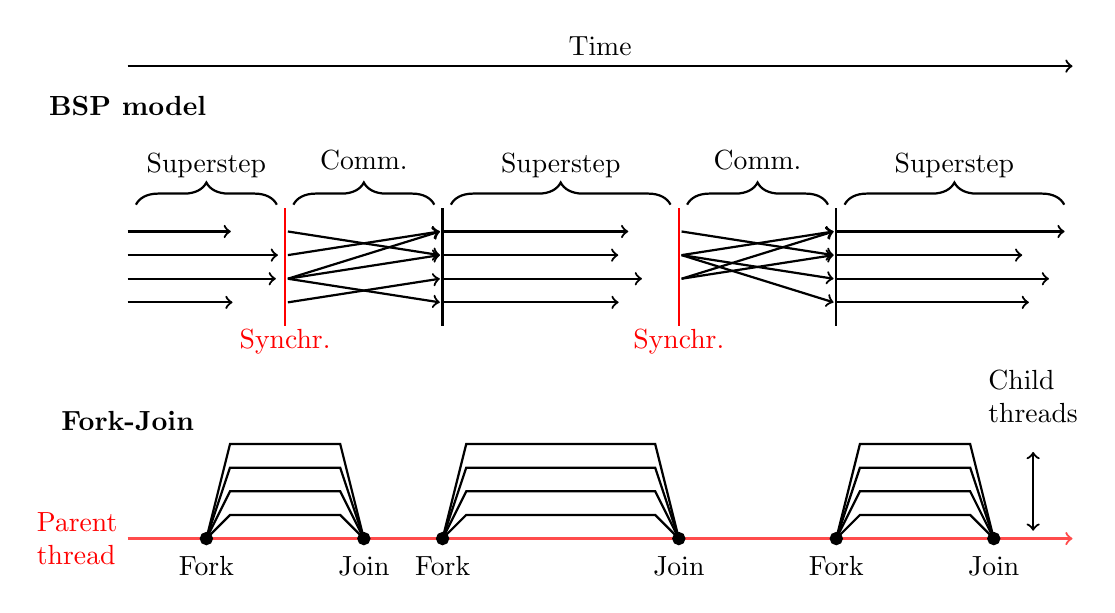
\begin{tikzpicture}[thick]
% Fork Join model
\coordinate (begin) at (0,0);
\coordinate (f0) at (1,0);
\coordinate (j0) at (3,0);

\coordinate (f1) at (4,0);
\coordinate (j1) at (7,0);

\coordinate (f2) at (9,0);
\coordinate (j2) at (11,0);

\coordinate (end) at (12,0);

\node at ([yshift=1.5cm]begin) {\textbf{Fork-Join}};


% Main threads and info
\draw[->,red!70] (0,0) -- (f0) -- (j0) -- (f1) -- (j1) -- (f2) -- (j2) -- (end);
\node[anchor=east,red,align=left] (0,0) {Parent\\thread};
\foreach \x in {0,...,2}{
\draw[fill,black,thick] (f\x) circle [radius=2pt] ;
\draw[fill,black,thick] (j\x) circle [radius=2pt] ;
\node at ([yshift=-10pt]f\x) {Fork}; 
\node at ([yshift=-10pt]j\x) {Join}; 
}

% Thread
\foreach \x in {1,...,4}{
  \draw[thick] (f0) -- ([yshift=\x*.3cm,xshift=.3cm]f0) -- ([xshift=-.3cm,yshift=\x*.3cm]j0) -- (j0);

  \draw[thick] (f1) -- ([yshift=\x*.3cm,xshift=.3cm]f1) -- ([xshift=-.3cm,yshift=\x*.3cm]j1) -- (j1);

  \draw[thick] (f2) -- ([yshift=\x*.3cm,xshift=.3cm]f2) -- ([xshift=-.3cm,yshift=\x*.3cm]j2) -- (j2);
}

% Name of threads
\draw[<->] (11.5,0.1) -- (11.5,1.1) node[anchor=south,yshift=7pt,align=left] {Child\\threads};


% BSP model
\coordinate (begin) at (0,3);

\coordinate (s0) at (2,3);
\coordinate (c0) at (4,3);
\coordinate (s1) at (7,3);
\coordinate (c1) at (9,3);
%\coordinate (s2) at (9,3);

\coordinate (end) at (12,3);

% Figure name 
\node at ([yshift=2.5cm]begin) {\textbf{BSP model}};

\draw [decorate,decoration={brace,amplitude=8pt,raise=4pt},yshift=0pt] ([yshift=1.1cm,xshift=3pt]begin) -- ([yshift=1.1cm,,xshift=-3pt]s0) node [black,midway,above,yshift=10pt] {Superstep};

\draw [decorate,decoration={brace,amplitude=8pt,raise=4pt},yshift=0pt] ([yshift=1.1cm,xshift=3pt]s0) -- ([yshift=1.1cm,,xshift=-3pt]c0) node [black,midway,above,yshift=13pt] {Comm.};

\draw [decorate,decoration={brace,amplitude=8pt,raise=4pt},yshift=0pt] ([yshift=1.1cm,xshift=3pt]c0) -- ([yshift=1.1cm,,xshift=-3pt]s1) node [black,midway,above,yshift=10pt] {Superstep};

\draw [decorate,decoration={brace,amplitude=8pt,raise=4pt},yshift=0pt] ([yshift=1.1cm,xshift=3pt]s1) -- ([yshift=1.1cm,,xshift=-3pt]c1) node [black,midway,above,yshift=13pt] {Comm.};

\draw [decorate,decoration={brace,amplitude=8pt,raise=4pt},yshift=0pt] ([yshift=1.1cm,xshift=3pt]c1) -- ([yshift=1.1cm,,xshift=-3pt]end) node [black,midway,above,yshift=10pt] {Superstep};


% Draw vertical lines 
\foreach \x in {0,...,1}{
\draw[red] ([yshift=-.3cm]s\x) -- ([yshift=1.2cm]s\x);
\node[red] at ([yshift=-.5cm]s\x) {Synchr.};

\draw ([yshift=-.3cm]c\x) -- ([yshift=1.2cm]c\x);
%\node at ([yshift=-.5cm]s\x) {Synchr.};
}

\foreach \x in {0,...,3}{
  \draw[->] ([yshift=\x*.3cm]begin) -- ([yshift=\x*.3cm,xshift=((rnd)*-20pt-2pt)]s0);
  \draw[->] ([yshift=\x*.3cm]c0) -- ([yshift=\x*.3cm,xshift=((rnd)*-20pt)-2pt]s1);
  \draw[->] ([yshift=\x*.3cm]c1) -- ([yshift=\x*.3cm,xshift=((rnd)*-20pt)-2pt]end);
  %\draw[->] ([yshift=\x*.3cm]s2) -- ([yshift=\x*.3cm,xshift=((rnd)*-20pt)-2pt]end);
}

% Add comms 
% comm 0 
\draw[->] ([xshift=1pt,yshift=.3cm]s0) -- ([xshift=-1pt,yshift=.9cm]c0);
\draw[->] ([xshift=1pt,yshift=0]s0) -- ([xshift=-1pt,yshift=.3cm]c0);
\draw[->] ([xshift=1pt,yshift=.3cm]s0) -- ([xshift=-1pt,yshift=0]c0);
\draw[->] ([xshift=1pt,yshift=.6cm]s0) -- ([xshift=-1pt,yshift=.9cm]c0);
\draw[->] ([xshift=1pt,yshift=.3cm]s0) -- ([xshift=-1pt,yshift=.6cm]c0);
\draw[->] ([xshift=1pt,yshift=.9cm]s0) -- ([xshift=-1pt,yshift=.6cm]c0);

% comm 1
\draw[->] ([xshift=1pt,yshift=.6cm]s1) -- ([xshift=-1pt,yshift=.9cm]c1);
\draw[->] ([xshift=1pt,yshift=.6cm]s1) -- ([xshift=-1pt,yshift=.3cm]c1);
\draw[->] ([xshift=1pt,yshift=.6cm]s1) -- ([xshift=-1pt,yshift=0]c1);
\draw[->] ([xshift=1pt,yshift=.3cm]s1) -- ([xshift=-1pt,yshift=.9cm]c1);
\draw[->] ([xshift=1pt,yshift=.3cm]s1) -- ([xshift=-1pt,yshift=.6cm]c1);
\draw[->] ([xshift=1pt,yshift=.9cm]s1) -- ([xshift=-1pt,yshift=.6cm]c1);


% Time 
\draw[->] ([yshift=3cm]begin) -- ([yshift=3cm]end) node[midway,above] {Time};

\end{tikzpicture}
\end{center}
\caption[BSP and Fork-Join model]{The Bulk Synchronous Parallel model and Fork-Join model, respectively top and bottom figure. The BSP is composed of computation steps, synchronizations and  exchanges in global communication steps. The Fork-Join model is based on a master thread that fork into sub-threads to delegate work and join them when the tasks are completed.} 
\label{fig:3_SOFT:bsp_fj}
\end{figure}

\subsection{Bulk Synchronous Parallelism }
\index{Bulk Synchronous Parallelism}
This model was presented in 1990 in \cite{valiant1990bridging}.
Being the link of HRAM and PRAM, the Bulk Synchronous Parallelism model is based on three elements:
\begin{itemize}[noitemsep,nolistsep]
  \item[-] a set of processor and their local memory;
  \item[-] a network for point-to-point communications between processors;
  \item[-] a unit allowing global synchronization and barriers.
\end{itemize}
This model is the most common on HPC clusters. 
It can be present event on node themselves: a process can be assign on a core or set of cores and the shared memory is separated between the processes. 
The synchronization can be hardware but in most cases it is handle by the runtime used.
A perfect example of runtime, presented later, is MPI. 

In this model the applications apply a succession of \textit{supersteps} separated by \textit{synchronizations} steps and data exchanges.

At opposite to H-PRAM which represent the execution as a succession of independent blocks working synchronously, BSP propose independent blocks of asynchronous applications synchronized by synchronization steps. 

In a communication/synchronization step we can consider the number of received messages $h_r$ and the number of send ones $h_s$.

The time lost in communication in one synchronization step is:
\begin{equation}
  T_{comm} = hg + I
\end{equation}

With $h = max(h_s,h_r)$, $g$ the time to transfer data and $I$ the start-up latency of the algorithm.
Indeed, the entry points and exit points of communications super-step can be a bottleneck considered in $I$.

The time for computing a super-step is: 
\begin{equation}
  T_{comp} = \frac{w}{r} + I
\end{equation}

With $w$ the maximum number of flops in the computation of this super-step, $r$ the speed of the CPU expressed in FLOPS and $I$ the start-up latency of the algorithm.
Indeed, the entry points and exit points of communications super-step can be a bottleneck considered in $I$.


The BSP model estimates the cost of one super-step with: 
\begin{equation}
  T_{comm} + T_{comp} = w + gh + 2l
\end{equation}

With $T$ a measure of time, a wall clock that measure elapsed time. 
We also note that usually $g$ and $I$ are function of the number of processes involved. 

It can then be use to compute the overall cost in BSP model summing all super-steps $s$: 
\begin{equation}
T = \sum_s \frac{max (w_s)}{r} + h_sg + I
\end{equation}

The problem of performances in this model can come from unequal repartitions of work, the load balancing. 
The processes with less than $w$ of work will be idle. 

\subsection{Fork-Join model}
\index{Fork-Join model}
The Fork-Join model or pattern is presented in figure~\ref{fig:3_SOFT:bsp_fj}.
A main thread pilot the overall execution. 
When requested by the application, typically following the idea of \textit{divide-and-conquer} approach, the main thread will fork and then join other threads. \index{Divide-and-conquer approach}
The \textit{Fork} operation, called by a logical thread parent, creates new logical threads children working in concurrency.
There is no limitations in the model and we find nested fork-join where a child can also call fork to generate sub-child and so on. 
The \textit{Join} can be called by both parents and child. Children call join when done and the parent join by wait until children completion.
The Fork operation increase concurrency and join decrease concurrency.

\section{Software/API}
In this section we present the main runtime, API and frameworks use in HPC and in this study in particular. 
The considered language will be C/C++, the most present in HPC world along with Fortran. 

\subsection{Shared memory programming}
\index{Unified Memory Access}
\index{Non Unified Memory Access}
On the supercomputers nodes we find one or several processors that access to UMA or NUMA memory. 
Several API and language provide tools to target and handle concurrency and data sharing in this context. 
The two main ones are PThreads and OpenMP for multi-core processors. 
We can also cite Cilk++ or TBB from Intel.

\subsubsection{PThreads}
\index{PThreads}
The Portable Operating System Interface (POSIX) threads API is an execution model based on threading interfaces. 
It is developed by the IEEE Computer Society. 
It allows the user to define threads that will execute concurrently on the processor resources using shared/private memory.
PThreads is the low level handling of threads and the user need to handle concurrency with semaphores, conditions variables and synchronization "by hand".
This makes the PThreads hard to use in complex applications and used only for very fine-grained control over the threads management. 

\begin{figure}[t!]
\begin{lstlisting}[language=C]
...
int min_val = MAX;
#pragma omp parallel for reduction(min:min_val)
for(int i = 0 ; i < X ; ++i){
	min_val = arr[i]<min_val?arr[i]:min_val;
}
...
\end{lstlisting}
\caption[OpenMP Reduction code]{OpenMP reduction code to compute minimum. Each thread search for the smallest value in a sub-set of the overall array. The reduction from the local minimum is then handle by the API.}
\label{code:openmp_reduction}
\end{figure}


\subsubsection{OpenMP}
\index{OpenMP}
\index{Unified Memory Access}
\index{Cache-Coherency Non Unified Memory Access}
\index{Fork-Join model}
Open Multi-Processing, OpenMP\footnote{http://www.openmp.org}~\cite{chapman2008using,supinski2017scaling,CDK+00}, is an API for multi-processing shared memory like UMA and CC-NUMA.
It is available in C/C++ and Fortran.
The user is provided with pragmas and functions to declare parallel loop and regions in the code. 
In this model the main thread, the first one before forks, command the fork-join operations. 

The last versions of OpenMP 4.0 also allow the user to target accelerators. 
During compilation the user specify on which processor or accelerator the code will be executed in parallel. 

We use OpenMP as a basis for the implementation of our CPU algorithms. 
Perfect for loop parallelization and parallel sections, we show that we can have the best results for CPU algorithms in most of the case. 
In our case, OpenMP is always use on the node to target all the processors cores in the shared memory. 

We note that the new versions of OpenMP also allows to target directly accelerators like NVIDIA ones. 

The code corresponding to a reduction using OpenMP API is presented on figure~\ref{code:openmp_reduction}.
This is linked with the PRAM model reduction presented at the beginning of this part. 

\subsection{Distributed programming}
In the cluster once the code have been developed locally and using the multiple cores available, the new step is to distribute it all over the nodes of the cluster. 
This step requires the processes to access NoRMA memory from a node to another. 
Several runtime are possible for this purpose and concerning our study. 
We should also cite HPX, the C++ standard distribution library, or AMPI for Adaptive MPI, Multi-Processor Computing (MPC) from CEA, etc.

\subsubsection{MPI}
\index{Message Passing Interface}
The Message Passing Interface, MPI, is the most famous runtime for distributed computing~\cite{gropp2014using,gropp2015using}.
Several implementations exists from Intel MPI\footnote{https://software.intel.com/en-us/intel-mpi-library} (IMPI), MVAPICH\footnote{http://mvapich.cse.ohio-state.edu/} by the Ohio State University and OpenMP\footnote{http://www.open-mpi.org} combining several MPI work like Los Alamos MPI (LA-MPI).
Those implementation follow the MPI standards 1.0, 2.0 or the latest, 3.0. 

This runtime provides directs, collectives and asynchronous functions for process(es) to process(es) communication.
A process can be a whole node or one or several cores on a processor.  

Some MPI implementations offer a support for accelerators targeting directly their memory through the network without multiple copies on host memory. 
The data go through one GPU to the other through network and PCIe.
This feature is used in our code in part 2 and 3.

Most of our code presented here are based on MPI for the distribution on the cluster. 
The advantage is its presence on all the cluster and the control over the data transfers. 

\begin{figure}
\begin{center}
\includegraphics[width=.8\textwidth]{\locpath/figures/chap1/GPUDirectRDMA.png}
\caption[GPUDirect RDMA from NVIDIA]{GPUDirect RDMA from NVIDIA Developer Blog: \textit{An Introduction to CUDA-Aware MPI}. On the right, without GPUDirect RDMA, the data have to be copied multiple times from GPU to CPU and then reach the network. On the left, by using GPUDirect RDMA, the data can directly be send on the network without extra copies.}
\label{fig:1_HPC:gpudirect_rdma}
\end{center}
\end{figure}

For NVIDIA this technology is called GPUDirect RDMA and presented on figure~\ref{fig:1_HPC:gpudirect_rdma}. 

In term of development MPI can be very efficient if use carefully. 
Indeed, the collectives communications such as \textit{MPI\_Alltoall}, \textit{MPI\_Allgather}, etc. can be a bottleneck when scaling up to thousands of processes. 
A specific care have to be taken in those implementation with privilege to asynchronous communications to hide computation than synchronous idle CPU time. 

\subsubsection{Charm++}
\index{Charm++}
Charm++\footnote{http://charmplusplus.org/} is an API for distributed programming developed by the University of Illinois Urbana-Champaign.
It is asynchronous messages paradigm driven.
In contrary of runtime like MPI that are synchronous but can handle asynchronous, Charm++ is natively asynchronous. 
It is based on \textit{chare object} that can be activated in response to messages from other \textit{chare objects} with triggered actions and callbacks. 
The repartition of data to processors is completely done by the API, the user just have to define correctly the partition and functions of the program. 
Charm++ also provides a GPU manager implementing data movement, asynchronous kernel launch, callbacks, etc.

A perfect example can be the hydrodynamics N-body simulation code Charm++ N-body Gravity Solver, ChaNGa~\cite{jetley2010scaling}, implemented with Charm++ and GPU support. 

\subsubsection{Legion}
\index{Legion}
Legion\footnote{http://legion.stanford.edu/} is a distributed runtime support by Stanford University, Los Alamos National Laboratory (LANL) and NVIDIA. 
This runtime is data-centered targeting distributed heterogeneous architectures. 
Data-centered runtime focuses to keep the data dependency and locality moving the tasks to the data and moving data only if requested. 
In this runtime the user defines data organization, partitions, privileges and coherency. 
Many aspect of the distribution and parallelization are then handle by the runtime itself.

The FleCSI runtime develops at LANL provide a template framework for multi-physics applications and is built on top of Legion. 
We give more details on this project and Legion on part 3.  

\subsection{Accelerators}
In order to target accelerators like GPU, several specific API have been developed. 
At first they were targeted for matrix computation with OpenGL or DirectX through specific devices languages to change the first purpose of the graphic pipeline. 
The GPGPUs arriving forced an evolution and new dedicated language to appear. 

\begin{figure}[t!]
\begin{lstlisting}[language=C]
__inline__ __device__ void warpReduceMin(int& val, int& idx)
{
    for (int offset = warpSize / 2; offset > 0; offset /= 2) {
        int tmpVal = __shfl_down(val, offset);
        int tmpIdx = __shfl_down(idx, offset);
        if (tmpVal < val) {
            val = tmpVal;
            idx = tmpIdx;
        }
    }
}
\end{lstlisting}
\caption[CUDA kernel for reduction]{CUDA kernel for reduction of minimum, the same example as with OpenMP code. The reduction is performed exactly as presented in the PRAM model, the domain is divided by 2 successively to reach the minimum on the thread 0. This operation is realised at WARP size in this example. }
\label{code:cuda_reduction}
\end{figure}

\subsubsection{CUDA}
\label{sec:CUDA}
\index{CUDA}
\index{NVIDIA}
The Compute Device Unified Architecture is the API develop in C/C++ Fortran by NVIDIA to target its GPGPUs. 
The API provide high and low level functions. 
The driver API allows a fine grain control over the executions.

The CUDA compiler is called NVidia C Compiler, NVCC. 
It converts the device code into Parallel Thread eXecution, PTX, and rely to the C++ host compiler for host code. 
PTX is a pseudo assembly language translated by the GPU in binary code that is then execute. 
As the ISA is simpler than CPU ones and able the user to work directly in assembly for very fine grain optimizations. 

\begin{figure*}[t!]
\centering
\setlength\fboxsep{0pt}
\setlength\fboxrule{0.25pt}
\includegraphics[scale=0.6]{\locpath/figures/chap1/smx}
\caption[NVIDIA GPU architecture and CUDA paradigms]{NVIDIA GPU and CUDA architecture overview. The right figure presents a logical view of the architecture of the GPU with the SMs, the processor, memory position. The left figure provides the CUDA paradigms to divide the threads in blocks and the blocks in a grid. The grid is at GPU level, the block is at SM level and the threads are at core level.}
 \label{fig:chap1_gpu}
%\vspace{-0.8cm} 
\end{figure*}

As presented in figure~\ref{fig:chap1_gpu}, NVIDIA GPUs include many \emph{Streaming Multiprocessors} (SM), each of which is composed of many \emph{Streaming Processors} (SP). In the Kepler architecture, the SM new generation is called SMX.
%
%In the CUDA programing model~\cite{cuda}, the GPU works as a SIMT co-processor of a conventional CPU. 
Grouped into \emph{blocks}, \textit{threads} execute \emph{kernels} functions synchronously.
Threads within a block can cooperate by sharing data on an SMX and synchronizing their execution to coordinate memory accesses; inside a block, the scheduler organizes \emph{warps} of 32 threads which execute the instructions simultaneously.
The blocks are distributed over the GPU SMXs to be executed independently.

%Memory, bandwidth and streams:
In order to use data in a device kernel, it has to be first created on the CPU, allocated on the GPU and then transferred from the CPU to the GPU; after the kernel execution, the results have to be transferred back from the GPU to the CPU. 
GPUs consist of several memory categories, organized hierarchically and differing by size, bandwidth and latency.   
On the one hand, the device's main memory is relatively large but has a slow access time due to a huge latency. 
On the other hand, each SMX has a small amount of shared memory and L1 cache, accessible by its SPs, with faster access, and registers organized as an SP-local memory. 
SMXs also have a constant memory cache and a texture memory cache.
%, that are linked to the constant and texture memories physically located in the device memory: these are read-only and have faster access time than the rest of the memory categories.
Reaching optimal computing efficiency requires considerable effort while programming.
Most of the global memory latency can then be hidden by the threads scheduler if there is enough computational effort to be executed while waiting for the global memory access to complete. Another way to hide this latency is to use streams to overlap kernel computation and memory load. 

%Threads synchronization:
It is also important to note that branching instructions may break the threads synchronous execution inside a warp and thus affect the program efficiency. 
This is the reason why test-based applications, like combinatorial problems that are inherently irregular, are considered as bad candidates for GPU implementation.\\ 
%This is particularly true with regard to combinatorial problems resolution. 
%Thus we intend to provide a way to regularize their execution, in order to get good acceleration with GPU computation. 

Specific tools have been made for HPC in the NVIDIA GPGPUs. 
\begin{description}[noitemsep,nolistsep]
  \item[Dynamic Parallelism] This feature allow the GPU kernels to run other kernels themselves. When more sub-tasks have to be generated this can be done directly on the GPU using dynamic parallelism.
  \item[Hyper-Q] This technology enable several CPU threads to execute kernels on the same GPU simultaneously. This can help to reduce the synchronization time and idle time of CPU cores for specific applications.
  \item[NVIDIA GPU-Direct] GPUs' memory and CPU ones are different and the Host much push the data on GPU before allowing it to compute. GPU-Direct allows direct transfers from GPU devices through the network. Usually implemented using MPI.  
\end{description}

Indeed, working with a very low level API like CUDA can lead to better performances. 
This can be very costly in development time. 
Regarding the time involved in coding compared to the performances gain, one may consider to use higher levels API like OpenACC. 

The reduction using the CUDA API is presented on figure~\ref{code:cuda_reduction}.
It shows, compared to OpenMP, the complexity of CUDA code. 

\subsubsection{OpenCL}
\index{OpenCL}
OpenCL is a multi-platform framework targeting a large part of nowadays architectures from processors to GPUs, FPGAs, etc.
A large group of company already provided conform version of the OpenCL standard: IBM, Intel, NVIDIA, AMD, ARM, etc.
This framework allows to produce a single code that can run in all the host or device architectures. 
It is quite similar to NVIDIA CUDA Driver API and based on kernels that are written and can be used in On-line/Off-line compilation meaning Just In Time (JIT) or not. 
The idea of OpenCL is great by rely on the vendors wrapper.
Indeed, one may wonder, what is the level of work done by NVIDIA on its own CUDA framework compare to the one done to implement OpenCL standards? 
What is the advantage for NVIDIA GPU to be able to be replace by another component and compare on the same level? 
Those questions are still empty but many tests prove that OpenCL can be as comparable as CUDA but rarely better\cite{karimi2010performance,fang2011comprehensive}. 

In this study most of the code had been developed using CUDA to have the best benefit of the NVIDIA GPUs present in the ROMEO Supercomputer. 
Also the long time partnership of the University of Reims Champagne-Ardenne and NVIDIA since 2003 allows us to exchange directly with the support and NVIDIA developers. 


\begin{figure}[t!]
\begin{lstlisting}[language=C]
...
int min_val = MAX; 
#pragma acc parallel loop copyin(arr[0:n]) reduction(min:min_val) 
for (int i=0; i<n; i++) { 
    min_val = arr[i]<min_val?arr[i]:min_val; 
}
...
\end{lstlisting}
\caption[OpenACC code for reduction]{OpenACC code for reduction of minimum. This example is very similar to the OpenMP code since OpenACC is following the same paradigm. The reduction will be handle directly on the GPU. }
\label{code:openacc_reduction}
\end{figure}


\subsubsection{OpenACC}
\index{OpenACC}
Open ACCelerators is a "user-driven directive-based performance-portable parallel programming model"\footnote{https://www.openacc.org/} developed with Cray, AMD, NVIDIA, etc.
This programming model propose, in a similar way to OpenMP, pragmas to define the loop parallelism and the device behavior. 
As the device memory is separated specific pragmas are use to define the memory movements.
Research works\cite{wienke2012openacc} tend to show that OpenACC performances are good regarding the time spend in the implementation itself compare to fine grain CUDA or OpenCL approaches. 
The little lack of performances can also be explain by the current contribution to companies in the wrapper for their architectures and devices. 

The reduction example is given on figure~\ref{code:openacc_reduction}. 
This shows the simplicity of writing accelerator code using high level API like OpenACC compared to the complex CUDA code. 
Indeed, this approach works in most of the case but for specific ones CUDA might outperform OpenACC. 

\begin{figure}
\centering 
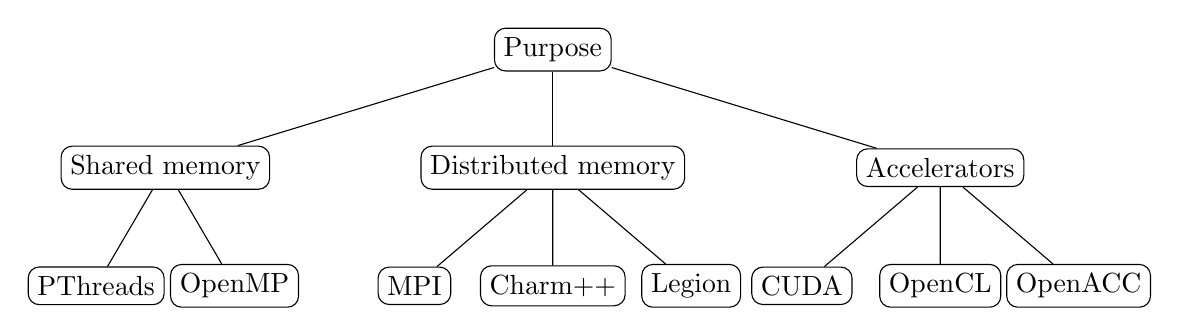
\begin{tikzpicture}[
  every node/.style = {
    level distance=1em,
    shape=rectangle, 
    rounded corners,
    draw, 
    align=center,
    top color=white%, 
   % bottom color=blue!20
  }]]
  \node {Purpose} [sibling distance=14em]
    child { node {Shared memory} [sibling distance=5em]
      child { node {PThreads}}
      child { node {OpenMP}}
    }
    child { node {Distributed memory} [sibling distance=5em]
        child{node {MPI}} 
        child{node {Charm++}}
        child{node {Legion}}
    }
    child { node {Accelerators} [sibling distance=5em]
      child {node  {CUDA}} 
      child { node {OpenCL}}
      child {node {OpenACC}}
    };
\end{tikzpicture}
\caption[Runtimes, libraries, framework and APIs]{Position of Runtimes, libraries, frameworks or APIs regarding their usage in HPC. We find shared memory, distributed memory and accelerator specific tools.}
\label{fig:1_HPC:software}
\end{figure}

The runtime, libraries, frameworks and APIs are summarized in figure~\ref{fig:1_HPC:software}.
They are used in combination. 
The usual one is MPI for distribution, OpenMP and CUDA to target processors and GPUs. 

%\section{Profiling tools}
%\todo{Est-ce interessant? Plus tard? Ne pas en parler?}
%\subsection{Intel suite}
%\subsection{MAQAO}
%\subsection{Allinea/MAP}

\section{Benchmarks}
\index{Benchmarks}
All those models, theory, hardware and software leads to better understanding and characterization of machines to produce better algorithm and solve bigger and harder problems. 
The question that arise is: how to know if a machine is better than another? 
We answer that question with FLOPS, IPC, OPS or just the frequency of the machine. 
The models like BSP or law's like Amdahl and Gustafson ones propose to find the best/worst case during the execution.

In real application the only way to really know what will be the behavior of a supercomputer is to try, test real code on it. 
This is call benchmarking.
Several kind of benchmarks exists and target a specific application of supercomputers. 
We present here the most famous benchmarks of HPC and their specificities.

\subsection{TOP500}
\index{TOP500}
The most famous benchmark is certainly the TOP500\footnote{http://www.top500.org}. 
It gives the ranking of the 500 most powerful, known, supercomputers of the world as its name indicates.
Since 1993 the organization assembles and maintains this list updated twice a year in June and November.

This benchmark is based on the LINPACK\cite{dongarra1994top500} a benchmark introduced by Jack J. Dongarra.\index{LINPACK}
This benchmark rely on solving  dense system of linear equations. 
As specified in this document this benchmark is just one of the tools to define the performance of a supercomputer. 
It reflects "the performance of a dedicated system for solving a dense system of linear equations".
This kind of benchmark is very regular in computation giving high results for FLOPS. 

In 1965 the Intel co-fonder Gordon Moore made an observation\cite{present2000cramming} on the evolution of devices. 
He pointed the fact that the number of transistors in a dense integrated circuit doubles approximately every eighteen months.
This is know as the Moore's law. 
Looking at the last TOP500 figure presented on figure~\ref{fig:intro_top500}, in the introduction of this document, we saw that nowadays machines does not fit in the law anymore. 
This is due to the size of transistor and the energy needed to reach more powerful machines. 
The Moore's law have been sustains by the arrival of many-cores architectures such as GPU or Xeon Phi. 
Tomorrow machines architectures will have to be based on hybrid with more paradigms and tools to take part of massive parallelism.


\subsection{Green500}
\index{Green500}
\index{PEZY}
\index{NVIDIA}
In conjunction of the TOP500, the Green500\footnote{https://www.top500.org/green500/} focus on the energy consumption of supercomputers. 
The scale is based on FLOPS per watts~\cite{feng2007green500}.
Indeed the energy wall is the main limitation for next generation and exascale supercomputers. 
In the last list, November 2017, the TOP3 machines are accelerated with PEZY-SC many-core devices. 
The TOP20 supercomputers are all equipped with many-cores architectures: 5 with PEZY-SC, 14 with NVIDIA P100 and 1 with the Sunway many-core devices. 
This show clearly that the nowadays energy efficient solutions resides in many-core architecture and more than that, hybrid supercomputers. 

\subsection{GRAPH500}
\index{GRAPH500}
The GRAPH500\footnote{https://www.graph500.org/} benchmark\cite{murphy2010introducing} focus on irregular memory accesses, and communications.
The authors try to find ways to face the futures large-scale large-data problems and data-driven analysis.
This can be see as a complement of the TOP500 for data intensive applications.
The aim is to generate a huge graph to fill all the maximum memory on the machine and then operate either:
\begin{description}
  \item[BFS:] A Breadth-First Search which is an algorithm starting from a root and exploring recursively all the neighbors. 
  This requires a lot of irregular communications and memory accesses. 
  \item[SSSP:] A Single Source Shortest Path which is an algorithm searching the shortest path from one node to the others. 
  Like the BFS it has an irregular behavior but also requires to keep more data during the computation.
\end{description}

This benchmark will be detailed in Part II Chapter II in our benchmark suite. 

\subsection{HPCG}
\index{High Performance Conjugate Gradient}
The High Performance Conjugate Gradient benchmark\footnote{http://www.hpcg-benchmark.org/} is a new benchmark created in 2015 and presented for the first time at SuperComputing 2015. 
The last list, November 2017 contains 115 supercomputers ranked. 
The list also offer to compare the results of Linpack compared to Conjugate Gradient. 
This benchmark is a first implementation of having both computation and 
communications aspects of HPC in the same test. 

This benchmark is presented and features:
\begin{itemize}[noitemsep,nolistsep]
\item[-] Sparse matrix-vector multiplication;
\item[-] Vector updates;
\item[-] Global dot products;
\item[-] Local symmetric Gauss-Seidel smoother;
\item[-] Sparse triangular solve (as part of the Gauss-Seidel smoother);
\item[-] Driven by multigrid preconditioned conjugate gradient algorithm that exercises the key kernels on a nested set of coarse grids;
\item[-] Reference implementation is written in C++ with MPI and OpenMP support.\\
\end{itemize}

\subsection{SPEC}
\index{SPEC Benchmark}
The \textit{Standard Performance Evaluation Corporation} is a non-profit corporation that provides benchmarks for a wide range of architectures. 
The benchmark proposes a specific set of tests for HPC.
The SPEC ACCEL, SPEC MPI and SPEC OMP are focused on OpenCL, OpenACC, MPI and OpenMP API, respectively. 
In every case multiple sub-benchmarks are proposed to target a large set of limitation like computational or data-intensive problems. 
The benchmark is done to be representative of "real life" problems. 

A recent study~\cite{8430508} shows through the utilization of this benchmark the art of supercomputers with the current limitations. 
It also shows which can be the solution for future machine and to reach the Exascale.\\

The benchmarks presented in this section are the most famous of HPC world. 
Indeed, they are not the perfect representative of the nowadays application or does not fit our need for optimized GPU using CUDA. 
The upcoming of big data and artificial intelligence in addition to classical "real life" applications impose HPC to evolute and find new ways to target new architectures. 
The TOP500 target the computational problem but does not handle a lot of irregularity. 
Indeed, solving dense linear equation is straight forward and also use the memory in a regular way.
The Graph500 is very interesting to focus on communication and does handle irregular behavior for communications and memory. 
The Green500 does target energy wall but can also be applied to any benchmark. 
The most interesting one may be the HPCG benchmark. 
It does create irregularity during computation and communication along to memory traversal. 

\section{Conclusion}
In this chapter we presented the most used software tools for HPC. 
From inside node with shared memory paradigms, accelerators and distributed memory using message passing runtime with asynchronous or synchronous behavior. 

The tools to target accelerators architectures tend to be less architecture dependent with API like OpenMP, OpenCL or OpenACC targeting all the machines architectures. 
Unfortunately the vendor themselves have to be involve to provide the best wrapper for their architecture. 
In the mean time vendor dependent API like CUDA for NVIDIA seems to deliver the best performances.

We show through the different benchmark that hybrid architecture start to have their place even in computation heavy and communication heavy context. 
They are the opportunity to reach exascale supercomputers in horizon 2020.  

The benchmarks we presented, the most famous ones, does not represent all the types of modern domain scientists problems. 
This study intents to provide a specific metrics representing computation and communication walls with highly irregular application. 
These tools will help us to show the real advantage of hybrid architectures over classical clusters.
